%% fig_ladder.tex   (generated by make_diagrams.py; do not edit by hand)
%% Betti numbers of an abelian fourfold as prisms, split into the Lefschetz image and the primitive part, with the hard Lefschetz arcs.
\documentclass[tikz,border=8pt]{standalone}
\usepackage{amsmath,amssymb}
\usetikzlibrary{arrows.meta,calc}
%% palette.tex -- shared colour definitions for the figures
\definecolor{PInk}{RGB}{26,32,44}
\definecolor{PBlue}{RGB}{37,82,139}
\definecolor{PTeal}{RGB}{23,127,125}
\definecolor{POchre}{RGB}{193,138,44}
\definecolor{PClay}{RGB}{178,74,58}
\definecolor{PSlate}{RGB}{108,122,137}
\definecolor{PViolet}{RGB}{110,86,150}
\definecolor{WBlue}{RGB}{223,234,246}
\definecolor{WTeal}{RGB}{220,238,236}
\definecolor{WOchre}{RGB}{250,240,218}
\definecolor{WClay}{RGB}{247,229,224}
\definecolor{WSlate}{RGB}{238,241,244}
\definecolor{PMag}{RGB}{158,58,110}
\definecolor{PGrass}{RGB}{62,124,66}
\definecolor{PAmber}{RGB}{214,112,38}
\definecolor{PIndigo}{RGB}{58,64,140}
\definecolor{PRule}{RGB}{176,186,197}

%% shared macros so the standalone figures match the paper
\providecommand{\QQ}{\mathbb{Q}}
\providecommand{\ZZ}{\mathbb{Z}}
\providecommand{\RR}{\mathbb{R}}
\providecommand{\CC}{\mathbb{C}}
\providecommand{\PP}{\mathbb{P}}
\providecommand{\Kx}{K^{\times}}
\providecommand{\HW}{W}
\providecommand{\Nm}{\mathrm{N}}
\providecommand{\Hdg}{\mathrm{Hdg}}
\providecommand{\NS}{\mathrm{NS}}
\providecommand{\cA}{\mathcal{A}}
\providecommand{\cD}{\mathcal{D}}
\providecommand{\cF}{\mathcal{F}}
\providecommand{\cP}{\mathcal{P}}
\providecommand{\cO}{\mathcal{O}}
\providecommand{\cQ}{\mathcal{Q}}
\providecommand{\bbar}[1]{\overline{#1}}
\providecommand{\ch}{\operatorname{ch}}
\providecommand{\End}{\mathrm{End}}

\begin{document}
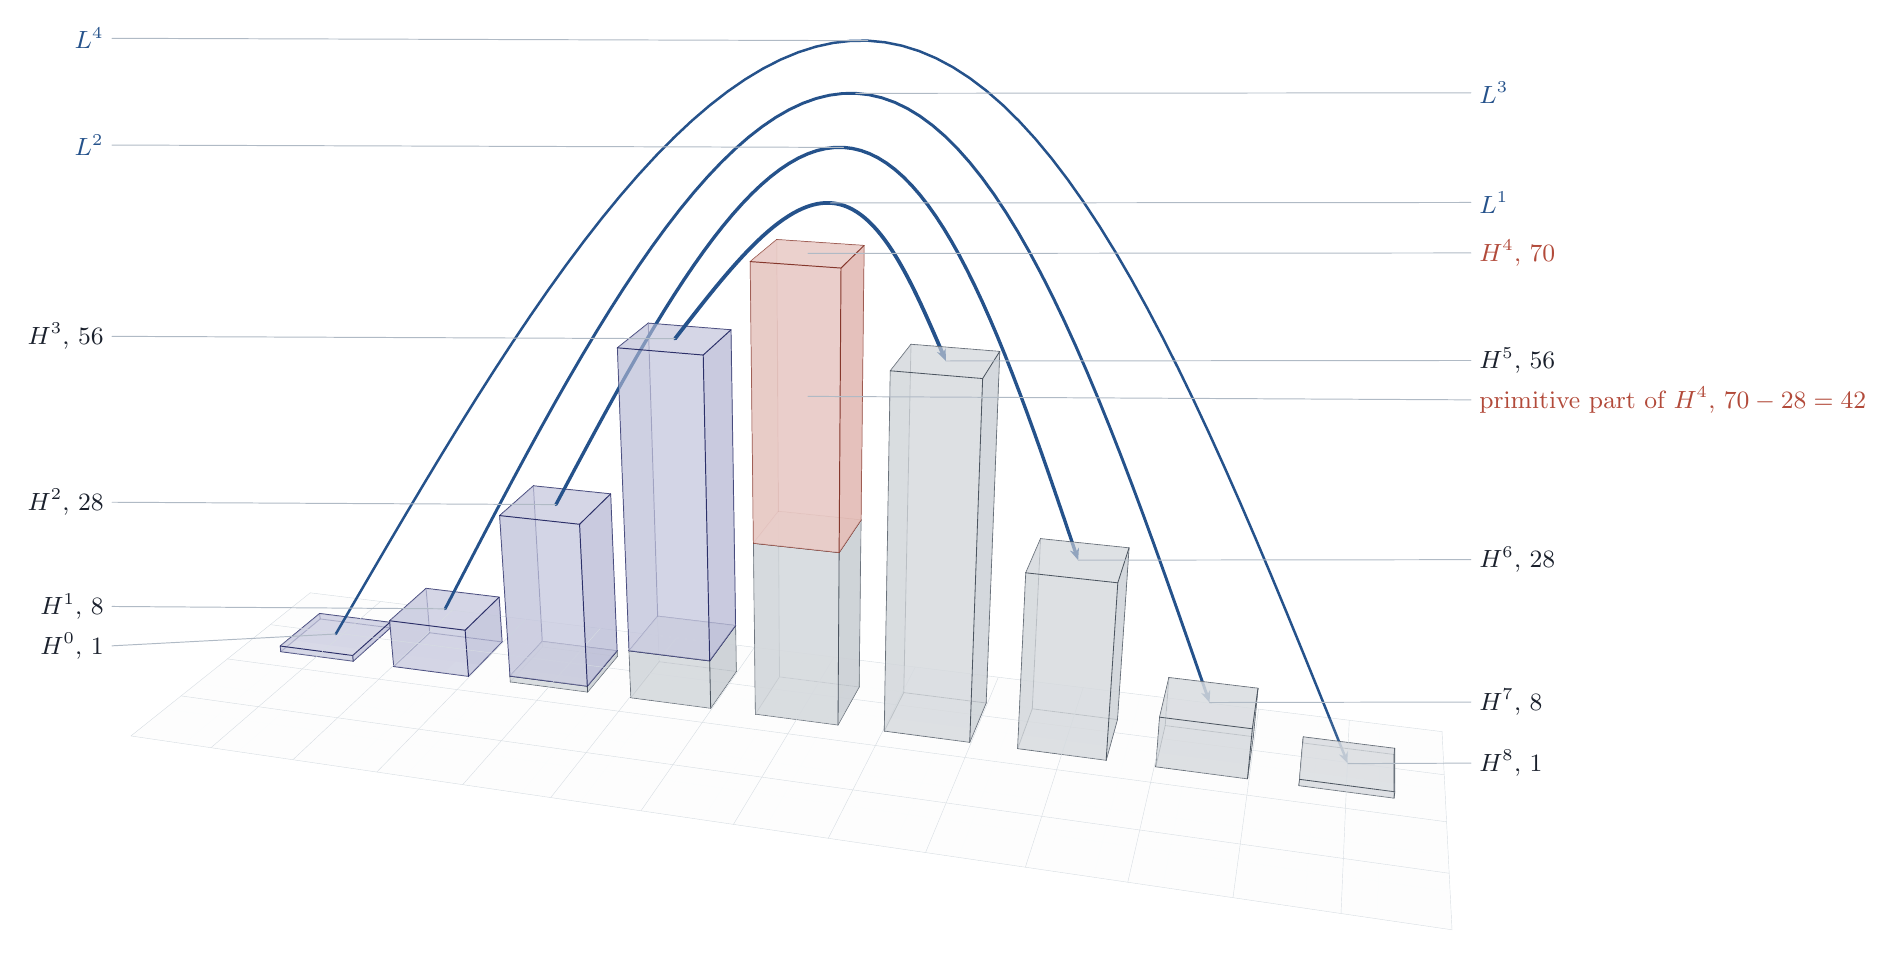
\begin{tikzpicture}[x=1cm,y=1cm,line join=round,line cap=round,
  font=\small,text=PInk]
  \path[draw=none,fill opacity=0.10,fill=PSlate!16!white] (-6.6553,-1.2051) -- (-6.0495,-1.2815) -- (-5.7283,-1.0117) -- (-6.3219,-0.9389) -- cycle;
  \path[draw=none,fill opacity=0.10,fill=PSlate!16!white] (-6.0495,-1.2815) -- (-5.4354,-1.3589) -- (-5.1268,-1.0854) -- (-5.7283,-1.0117) -- cycle;
  \path[draw=none,fill opacity=0.10,fill=PSlate!16!white] (-5.4354,-1.3589) -- (-4.8128,-1.4374) -- (-4.5172,-1.1602) -- (-5.1268,-1.0854) -- cycle;
  \draw[PIndigo!75!black,line width=0.35pt] (-6.1948,-1.2711) -- (-6.2020,-1.2021);
  \draw[PIndigo!75!black,line width=0.35pt] (-6.1948,-1.2711) -- (-5.3039,-1.3835);
  \path[draw=none,fill opacity=0.55,fill=PIndigo!28!white] (-6.1948,-1.2711) -- (-5.3039,-1.3835) -- (-5.3101,-1.3140) -- (-6.2020,-1.2021) -- cycle;
  \path[draw=none,fill opacity=0.10,fill=PSlate!16!white] (-4.8128,-1.4374) -- (-4.1816,-1.5170) -- (-3.8993,-1.2360) -- (-4.5172,-1.1602) -- cycle;
  \draw[PIndigo!75!black,line width=0.35pt] (-6.2020,-1.2021) -- (-5.3101,-1.3140);
  \path[draw=none,fill opacity=0.10,fill=PSlate!16!white] (-7.0054,-1.4846) -- (-6.3868,-1.5648) -- (-6.0495,-1.2815) -- (-6.6553,-1.2051) -- cycle;
  \draw[PIndigo!75!black,line width=0.35pt] (-5.3039,-1.3835) -- (-5.3101,-1.3140);
  \path[draw=none,fill opacity=0.10,fill=PSlate!16!white] (-4.1816,-1.5170) -- (-3.5415,-1.5977) -- (-3.2730,-1.3128) -- (-3.8993,-1.2360) -- cycle;
  \path[draw=none,fill opacity=0.10,fill=PSlate!16!white] (-6.3868,-1.5648) -- (-5.7596,-1.6462) -- (-5.4354,-1.3589) -- (-6.0495,-1.2815) -- cycle;
  \draw[PIndigo!75!black,line width=0.35pt] (-6.6944,-1.6858) -- (-6.1948,-1.2711);
  \path[draw=none,fill opacity=0.55,fill=PIndigo!37!white] (-6.6944,-1.6858) -- (-6.1948,-1.2711) -- (-6.2020,-1.2021) -- (-6.7024,-1.6148) -- cycle;
  \draw[PIndigo!75!black,line width=0.35pt] (-6.7024,-1.6148) -- (-6.2020,-1.2021);
  \path[draw=none,fill opacity=0.10,fill=PSlate!16!white] (-3.5415,-1.5977) -- (-2.8924,-1.6796) -- (-2.6381,-1.3907) -- (-3.2730,-1.3128) -- cycle;
  \draw[PIndigo!75!black,line width=0.35pt] (-4.8047,-1.4465) -- (-4.8503,-0.8831);
  \draw[PIndigo!75!black,line width=0.35pt] (-4.8047,-1.4465) -- (-3.8857,-1.5625);
  \path[draw=none,fill opacity=0.55,fill=PIndigo!26!white] (-6.6944,-1.6858) -- (-5.7755,-1.8067) -- (-5.3039,-1.3835) -- (-6.1948,-1.2711) -- cycle;
  \path[draw=none,fill opacity=0.10,fill=PSlate!16!white] (-5.7596,-1.6462) -- (-5.1234,-1.7287) -- (-4.8128,-1.4374) -- (-5.4354,-1.3589) -- cycle;
  \path[draw=none,fill opacity=0.55,fill=PIndigo!26!white] (-6.7024,-1.6148) -- (-5.7825,-1.7351) -- (-5.3101,-1.3140) -- (-6.2020,-1.2021) -- cycle;
  \path[draw=none,fill opacity=0.55,fill=PIndigo!28!white] (-4.8047,-1.4465) -- (-3.8857,-1.5625) -- (-3.9230,-0.9944) -- (-4.8503,-0.8831) -- cycle;
  \path[draw=none,fill opacity=0.10,fill=PSlate!16!white] (-2.8924,-1.6796) -- (-2.2341,-1.7626) -- (-1.9944,-1.4696) -- (-2.6381,-1.3907) -- cycle;
  \draw[PIndigo!75!black,line width=0.35pt] (-5.7755,-1.8067) -- (-5.3039,-1.3835);
  \path[draw=none,fill opacity=0.55,fill=PIndigo!37!white] (-5.7755,-1.8067) -- (-5.3039,-1.3835) -- (-5.3101,-1.3140) -- (-5.7825,-1.7351) -- cycle;
  \draw[PIndigo!75!black,line width=0.35pt] (-5.7825,-1.7351) -- (-5.3101,-1.3140);
  \draw[PIndigo!75!black,line width=0.35pt] (-4.8503,-0.8831) -- (-3.9230,-0.9944);
  \draw[PIndigo!75!black,line width=0.35pt] (-3.8857,-1.5625) -- (-3.9230,-0.9944);
  \path[draw=none,fill opacity=0.10,fill=PSlate!16!white] (-5.1234,-1.7287) -- (-4.4783,-1.8124) -- (-4.1816,-1.5170) -- (-4.8128,-1.4374) -- cycle;
  \draw[PSlate!70!black,line width=0.3pt] (-3.3707,-1.6275) -- (-3.3747,-1.5567);
  \path[draw=none,fill opacity=0.10,fill=PSlate!16!white] (-2.2341,-1.7626) -- (-1.5664,-1.8468) -- (-1.3418,-1.5497) -- (-1.9944,-1.4696) -- cycle;
  \draw[PIndigo!75!black,line width=0.35pt] (-5.2604,-1.8745) -- (-4.8047,-1.4465);
  \path[draw=none,fill opacity=0.10,fill=PSlate!16!white] (-7.3733,-1.7783) -- (-6.7415,-1.8627) -- (-6.3868,-1.5648) -- (-7.0054,-1.4846) -- cycle;
  \draw[PSlate!70!black,line width=0.3pt] (-3.3707,-1.6275) -- (-2.4223,-1.7471);
  \draw[PIndigo!75!black,line width=0.35pt] (-6.6944,-1.6858) -- (-6.7024,-1.6148);
  \path[draw=none,fill opacity=0.72,fill=PSlate!28!white] (-3.3707,-1.6275) -- (-2.4223,-1.7471) -- (-2.4253,-1.6758) -- (-3.3747,-1.5567) -- cycle;
  \draw[PSlate!70!black,line width=0.3pt] (-3.3747,-1.5567) -- (-2.4253,-1.6758);
  \draw[PIndigo!75!black,line width=0.35pt] (-3.3747,-1.5567) -- (-2.4253,-1.6758);
  \path[draw=none,fill opacity=0.10,fill=PSlate!16!white] (-4.4783,-1.8124) -- (-3.8238,-1.8974) -- (-3.5415,-1.5977) -- (-4.1816,-1.5170) -- cycle;
  \path[draw=none,fill opacity=0.55,fill=PIndigo!37!white] (-5.2604,-1.8745) -- (-4.8047,-1.4465) -- (-4.8503,-0.8831) -- (-5.3123,-1.2941) -- cycle;
  \path[draw=none,fill opacity=0.55,fill=PIndigo!26!white] (-5.2604,-1.8745) -- (-4.3116,-1.9993) -- (-3.8857,-1.5625) -- (-4.8047,-1.4465) -- cycle;
  \path[draw=none,fill opacity=0.10,fill=PSlate!16!white] (-1.5664,-1.8468) -- (-0.8891,-1.9322) -- (-0.6800,-1.6309) -- (-1.3418,-1.5497) -- cycle;
  \draw[PIndigo!75!black,line width=0.35pt] (-6.6944,-1.6858) -- (-5.7755,-1.8067);
  \path[draw=none,fill opacity=0.55,fill=PIndigo!28!white] (-6.6944,-1.6858) -- (-5.7755,-1.8067) -- (-5.7825,-1.7351) -- (-6.7024,-1.6148) -- cycle;
  \path[draw=none,fill opacity=0.10,fill=PSlate!16!white] (-6.7415,-1.8627) -- (-6.1005,-1.9484) -- (-5.7596,-1.6462) -- (-6.3868,-1.5648) -- cycle;
  \draw[PSlate!70!black,line width=0.3pt] (-2.4223,-1.7471) -- (-2.4253,-1.6758);
  \draw[PRule!50,line width=0.15pt] (-6.3219,-0.9389) -- (8.0522,-2.7019);
  \draw[PIndigo!75!black,line width=0.35pt] (-6.7024,-1.6148) -- (-5.7825,-1.7351);
  \draw[PIndigo!75!black,line width=0.35pt] (-5.3123,-1.2941) -- (-4.8503,-0.8831);
  \draw[PIndigo!75!black,line width=0.35pt] (-4.3116,-1.9993) -- (-3.8857,-1.5625);
  \draw[PRule!50,line width=0.15pt] (-8.5990,-2.7569) -- (-6.3219,-0.9389);
  \path[draw=none,fill opacity=0.10,fill=PSlate!16!white] (-3.8238,-1.8974) -- (-3.1599,-1.9835) -- (-2.8924,-1.6796) -- (-3.5415,-1.5977) -- cycle;
  \draw[PIndigo!75!black,line width=0.35pt] (-5.7755,-1.8067) -- (-5.7825,-1.7351);
  \path[draw=none,fill opacity=0.10,fill=PSlate!16!white] (-0.8891,-1.9322) -- (-0.2020,-2.0188) -- (-0.0088,-1.7132) -- (-0.6800,-1.6309) -- cycle;
  \path[draw=none,fill opacity=0.55,fill=PIndigo!26!white] (-5.3123,-1.2941) -- (-4.3545,-1.4140) -- (-3.9230,-0.9944) -- (-4.8503,-0.8831) -- cycle;
  \draw[PIndigo!75!black,line width=0.35pt] (-3.3747,-1.5567) -- (-3.4874,0.4192);
  \path[draw=none,fill opacity=0.55,fill=PIndigo!37!white] (-4.3116,-1.9993) -- (-3.8857,-1.5625) -- (-3.9230,-0.9944) -- (-4.3545,-1.4140) -- cycle;
  \path[draw=none,fill opacity=0.10,fill=PSlate!16!white] (-6.1005,-1.9484) -- (-5.4503,-2.0352) -- (-5.1234,-1.7287) -- (-5.7596,-1.6462) -- cycle;
  \draw[PSlate!70!black,line width=0.3pt] (-3.7795,-2.0693) -- (-3.3707,-1.6275);
  \path[draw=none,fill opacity=0.72,fill=PSlate!37!white] (-3.7795,-2.0693) -- (-3.3707,-1.6275) -- (-3.3747,-1.5567) -- (-3.7842,-1.9964) -- cycle;
  \draw[PSlate!70!black,line width=0.3pt] (-3.7842,-1.9964) -- (-3.3747,-1.5567);
  \draw[PIndigo!75!black,line width=0.35pt] (-3.7842,-1.9964) -- (-3.3747,-1.5567);
  \path[draw=none,fill opacity=0.10,fill=PSlate!16!white] (-3.1599,-1.9835) -- (-2.4864,-2.0709) -- (-2.2341,-1.7626) -- (-2.8924,-1.6796) -- cycle;
  \draw[PSlate!70!black,line width=0.3pt] (-1.8907,-1.8142) -- (-1.9093,-1.2362);
  \draw[PSlate!70!black,line width=0.3pt] (-1.8907,-1.8142) -- (-0.9116,-1.9378);
  \draw[PIndigo!75!black,line width=0.35pt] (-4.3545,-1.4140) -- (-3.9230,-0.9944);
  \path[draw=none,fill opacity=0.55,fill=PIndigo!28!white] (-3.3747,-1.5567) -- (-2.4253,-1.6758) -- (-2.5071,0.3171) -- (-3.4874,0.4192) -- cycle;
  \draw[PRule!50,line width=0.15pt] (-7.5824,-2.9061) -- (-5.4285,-1.0484);
  \path[draw=none,fill opacity=0.72,fill=PSlate!26!white] (-3.7795,-2.0693) -- (-2.7992,-2.1983) -- (-2.4223,-1.7471) -- (-3.3707,-1.6275) -- cycle;
  \path[draw=none,fill opacity=0.10,fill=PSlate!16!white] (-0.2020,-2.0188) -- (0.4951,-2.1068) -- (0.6719,-1.7967) -- (-0.0088,-1.7132) -- cycle;
  \path[draw=none,fill opacity=0.72,fill=PSlate!26!white] (-3.7842,-1.9964) -- (-2.8027,-2.1248) -- (-2.4253,-1.6758) -- (-3.3747,-1.5567) -- cycle;
  \path[draw=none,fill opacity=0.55,fill=PIndigo!26!white] (-3.7842,-1.9964) -- (-2.8027,-2.1248) -- (-2.4253,-1.6758) -- (-3.3747,-1.5567) -- cycle;
  \path[draw=none,fill opacity=0.10,fill=PSlate!16!white] (-5.4503,-2.0352) -- (-4.7905,-2.1234) -- (-4.4783,-1.8124) -- (-5.1234,-1.7287) -- cycle;
  \draw[PIndigo!75!black,line width=0.35pt] (-5.2604,-1.8745) -- (-5.3123,-1.2941);
  \path[draw=none,fill opacity=0.72,fill=PSlate!28!white] (-1.8907,-1.8142) -- (-0.9116,-1.9378) -- (-0.9206,-1.3549) -- (-1.9093,-1.2362) -- cycle;
  \draw[PIndigo!75!black,line width=0.35pt] (-5.2604,-1.8745) -- (-4.3116,-1.9993);
  \draw[PIndigo!75!black,line width=0.35pt] (-2.4253,-1.6758) -- (-2.5071,0.3171);
  \path[draw=none,fill opacity=0.10,fill=PSlate!16!white] (-2.4864,-2.0709) -- (-1.8030,-2.1596) -- (-1.5664,-1.8468) -- (-2.2341,-1.7626) -- cycle;
  \draw[PSlate!70!black,line width=0.3pt] (-2.7992,-2.1983) -- (-2.4223,-1.7471);
  \path[draw=none,fill opacity=0.10,fill=PSlate!16!white] (-7.7605,-2.0874) -- (-7.1148,-2.1763) -- (-6.7415,-1.8627) -- (-7.3733,-1.7783) -- cycle;
  \path[draw=none,fill opacity=0.72,fill=PSlate!37!white] (-2.7992,-2.1983) -- (-2.4223,-1.7471) -- (-2.4253,-1.6758) -- (-2.8027,-2.1248) -- cycle;
  \draw[PSlate!70!black,line width=0.3pt] (-2.8027,-2.1248) -- (-2.4253,-1.6758);
  \draw[PIndigo!75!black,line width=0.35pt] (-2.8027,-2.1248) -- (-2.4253,-1.6758);
  \path[draw=none,fill opacity=0.10,fill=PSlate!16!white] (0.4951,-2.1068) -- (1.2025,-2.1960) -- (1.3623,-1.8813) -- (0.6719,-1.7967) -- cycle;
  \draw[PSlate!70!black,line width=0.3pt] (-1.9093,-1.2362) -- (-0.9206,-1.3549);
  \draw[PIndigo!75!black,line width=0.35pt] (-1.9093,-1.2362) -- (-0.9206,-1.3549);
  \path[draw=none,fill opacity=0.55,fill=PIndigo!28!white] (-5.2604,-1.8745) -- (-4.3116,-1.9993) -- (-4.3545,-1.4140) -- (-5.3123,-1.2941) -- cycle;
  \draw[PSlate!70!black,line width=0.3pt] (-0.9116,-1.9378) -- (-0.9206,-1.3549);
  \path[draw=none,fill opacity=0.10,fill=PSlate!16!white] (-4.7905,-2.1234) -- (-4.1211,-2.2128) -- (-3.8238,-1.8974) -- (-4.4783,-1.8124) -- cycle;
  \draw[PRule!50,line width=0.15pt] (-6.5418,-3.0588) -- (-4.5172,-1.1602);
  \draw[PSlate!70!black,line width=0.3pt] (-2.2493,-2.2706) -- (-1.8907,-1.8142);
  \path[draw=none,fill opacity=0.10,fill=PSlate!16!white] (-1.8030,-2.1596) -- (-1.1094,-2.2495) -- (-0.8891,-1.9322) -- (-1.5664,-1.8468) -- cycle;
  \draw[PIndigo!75!black,line width=0.35pt] (-5.3123,-1.2941) -- (-4.3545,-1.4140);
  \path[draw=none,fill opacity=0.55,fill=PIndigo!37!white] (-3.7842,-1.9964) -- (-3.3747,-1.5567) -- (-3.4874,0.4192) -- (-3.9155,0.0419) -- cycle;
  \draw[PIndigo!75!black,line width=0.35pt] (-4.3116,-1.9993) -- (-4.3545,-1.4140);
  \path[draw=none,fill opacity=0.10,fill=PSlate!16!white] (-7.1148,-2.1763) -- (-6.4596,-2.2666) -- (-6.1005,-1.9484) -- (-6.7415,-1.8627) -- cycle;
  \draw[PSlate!70!black,line width=0.3pt] (-0.3626,-2.0071) -- (0.6489,-2.1347);
  \draw[PSlate!70!black,line width=0.3pt] (-3.7795,-2.0693) -- (-3.7842,-1.9964);
  \path[draw=none,fill opacity=0.10,fill=PSlate!16!white] (1.2025,-2.1960) -- (1.9204,-2.2865) -- (2.0627,-1.9673) -- (1.3623,-1.8813) -- cycle;
  \draw[PIndigo!75!black,line width=0.35pt] (-3.4874,0.4192) -- (-2.5071,0.3171);
  \path[draw=none,fill opacity=0.10,fill=PSlate!16!white] (-4.1211,-2.2128) -- (-3.4417,-2.3036) -- (-3.1599,-1.9835) -- (-3.8238,-1.8974) -- cycle;
  \path[draw=none,fill opacity=0.72,fill=PSlate!37!white] (-2.2493,-2.2706) -- (-1.8907,-1.8142) -- (-1.9093,-1.2362) -- (-2.2722,-1.6747) -- cycle;
  \path[draw=none,fill opacity=0.72,fill=PSlate!26!white] (-2.2493,-2.2706) -- (-1.2359,-2.4039) -- (-0.9116,-1.9378) -- (-1.8907,-1.8142) -- cycle;
  \path[draw=none,fill opacity=0.10,fill=PSlate!16!white] (-1.1094,-2.2495) -- (-0.4056,-2.3409) -- (-0.2020,-2.0188) -- (-0.8891,-1.9322) -- cycle;
  \draw[PSlate!70!black,line width=0.3pt] (-3.7795,-2.0693) -- (-2.7992,-2.1983);
  \path[draw=none,fill opacity=0.72,fill=PSlate!28!white] (-3.7795,-2.0693) -- (-2.7992,-2.1983) -- (-2.8027,-2.1248) -- (-3.7842,-1.9964) -- cycle;
  \draw[PSlate!70!black,line width=0.3pt] (-3.7842,-1.9964) -- (-2.8027,-2.1248);
  \draw[PIndigo!75!black,line width=0.35pt] (-3.7842,-1.9964) -- (-2.8027,-2.1248);
  \path[draw=none,fill opacity=0.10,fill=PSlate!16!white] (-6.4596,-2.2666) -- (-5.7946,-2.3581) -- (-5.4503,-2.0352) -- (-6.1005,-1.9484) -- cycle;
  \draw[PSlate!70!black,line width=0.3pt] (-2.2722,-1.6747) -- (-1.9093,-1.2362);
  \draw[PIndigo!75!black,line width=0.35pt] (-2.2722,-1.6747) -- (-1.9093,-1.2362);
  \draw[PSlate!70!black,line width=0.3pt] (-1.2359,-2.4039) -- (-0.9116,-1.9378);
  \draw[PRule!50,line width=0.15pt] (-5.4763,-3.2151) -- (-3.5872,-1.2743);
  \path[draw=none,fill opacity=0.10,fill=PSlate!16!white] (1.9204,-2.2865) -- (2.6490,-2.3784) -- (2.7733,-2.0544) -- (2.0627,-1.9673) -- cycle;
  \path[draw=none,fill opacity=0.10,fill=PSlate!16!white] (-3.4417,-2.3036) -- (-2.7522,-2.3957) -- (-2.4864,-2.0709) -- (-3.1599,-1.9835) -- cycle;
  \path[draw=none,fill opacity=0.55,fill=PIndigo!37!white] (-2.8027,-2.1248) -- (-2.4253,-1.6758) -- (-2.5071,0.3171) -- (-2.9010,-0.0685) -- cycle;
  \draw[PSlate!70!black,line width=0.3pt] (-2.7992,-2.1983) -- (-2.8027,-2.1248);
  \draw[PSlate!70!black,line width=0.3pt] (-0.3626,-2.0071) -- (-0.3755,0.0951);
  \path[draw=none,fill opacity=0.10,fill=PSlate!16!white] (-0.4056,-2.3409) -- (0.3088,-2.4336) -- (0.4951,-2.1068) -- (-0.2020,-2.0188) -- cycle;
  \draw[PRule!50,line width=0.15pt] (-6.8282,-1.3431) -- (8.0798,-3.2498);
  \path[draw=none,fill opacity=0.72,fill=PSlate!26!white] (-2.2722,-1.6747) -- (-1.2486,-1.8029) -- (-0.9206,-1.3549) -- (-1.9093,-1.2362) -- cycle;
  \path[draw=none,fill opacity=0.55,fill=PIndigo!26!white] (-2.2722,-1.6747) -- (-1.2486,-1.8029) -- (-0.9206,-1.3549) -- (-1.9093,-1.2362) -- cycle;
  \path[draw=none,fill opacity=0.72,fill=PSlate!37!white] (-1.2359,-2.4039) -- (-0.9116,-1.9378) -- (-0.9206,-1.3549) -- (-1.2486,-1.8029) -- cycle;
  \draw[PSlate!70!black,line width=0.3pt] (-0.6673,-2.4787) -- (-0.3626,-2.0071);
  \path[draw=none,fill opacity=0.10,fill=PSlate!16!white] (-5.7946,-2.3581) -- (-5.1197,-2.4511) -- (-4.7905,-2.1234) -- (-5.4503,-2.0352) -- cycle;
  \path[draw=none,fill opacity=0.10,fill=PSlate!16!white] (2.6490,-2.3784) -- (3.3885,-2.4716) -- (3.4943,-2.1428) -- (2.7733,-2.0544) -- cycle;
  \draw[PIndigo!75!black,line width=0.35pt] (-3.9155,0.0419) -- (-3.4874,0.4192);
  \draw[PSlate!70!black,line width=0.3pt] (1.2162,-2.2063) -- (2.2617,-2.3382);
  \path[draw=none,fill opacity=0.10,fill=PSlate!16!white] (-2.7522,-2.3957) -- (-2.0523,-2.4893) -- (-1.8030,-2.1596) -- (-2.4864,-2.0709) -- cycle;
  \path[draw=none,fill opacity=0.72,fill=PSlate!28!white] (-0.3626,-2.0071) -- (0.6489,-2.1347) -- (0.6724,-0.0141) -- (-0.3755,0.0951) -- cycle;
  \draw[PSlate!70!black,line width=0.3pt] (-1.2486,-1.8029) -- (-0.9206,-1.3549);
  \draw[PIndigo!75!black,line width=0.35pt] (-1.2486,-1.8029) -- (-0.9206,-1.3549);
  \draw[PIndigo!75!black,line width=0.35pt] (-3.7842,-1.9964) -- (-3.9155,0.0419);
  \draw[PIndigo!75!black,line width=0.35pt] (-1.9093,-1.2362) -- (-2.0287,2.4852);
  \path[draw=none,fill opacity=0.10,fill=PSlate!16!white] (-8.1685,-2.4132) -- (-7.5084,-2.5069) -- (-7.1148,-2.1763) -- (-7.7605,-2.0874) -- cycle;
  \draw[PRule!50,line width=0.15pt] (-4.3850,-3.3752) -- (-2.6381,-1.3907);
  \path[draw=none,fill opacity=0.72,fill=PSlate!26!white] (-0.6673,-2.4787) -- (0.3809,-2.6166) -- (0.6489,-2.1347) -- (-0.3626,-2.0071) -- cycle;
  \path[draw=none,fill opacity=0.10,fill=PSlate!16!white] (0.3088,-2.4336) -- (1.0340,-2.5277) -- (1.2025,-2.1960) -- (0.4951,-2.1068) -- cycle;
  \path[draw=none,fill opacity=0.55,fill=PIndigo!26!white] (-3.9155,0.0419) -- (-2.9010,-0.0685) -- (-2.5071,0.3171) -- (-3.4874,0.4192) -- cycle;
  \path[draw=none,fill opacity=0.10,fill=PSlate!16!white] (-5.1197,-2.4511) -- (-4.4345,-2.5455) -- (-4.1211,-2.2128) -- (-4.7905,-2.1234) -- cycle;
  \draw[PSlate!70!black,line width=0.3pt] (-2.2493,-2.2706) -- (-2.2722,-1.6747);
  \draw[PSlate!70!black,line width=0.3pt] (-2.2493,-2.2706) -- (-1.2359,-2.4039);
  \draw[PSlate!70!black,line width=0.3pt] (0.6489,-2.1347) -- (0.6724,-0.0141);
  \path[draw=none,fill opacity=0.10,fill=PSlate!16!white] (3.3885,-2.4716) -- (4.1392,-2.5663) -- (4.2260,-2.2326) -- (3.4943,-2.1428) -- cycle;
  \path[draw=none,fill opacity=0.55,fill=PIndigo!28!white] (-3.7842,-1.9964) -- (-2.8027,-2.1248) -- (-2.9010,-0.0685) -- (-3.9155,0.0419) -- cycle;
  \path[draw=none,fill opacity=0.55,fill=PIndigo!28!white] (-1.9093,-1.2362) -- (-0.9206,-1.3549) -- (-0.9788,2.4007) -- (-2.0287,2.4852) -- cycle;
  \path[draw=none,fill opacity=0.10,fill=PSlate!16!white] (-2.0523,-2.4893) -- (-1.3417,-2.5842) -- (-1.1094,-2.2495) -- (-1.8030,-2.1596) -- cycle;
  \draw[PSlate!70!black,line width=0.3pt] (0.3809,-2.6166) -- (0.6489,-2.1347);
  \path[draw=none,fill opacity=0.10,fill=PSlate!16!white] (-7.5084,-2.5069) -- (-6.8383,-2.6022) -- (-6.4596,-2.2666) -- (-7.1148,-2.1763) -- cycle;
  \draw[PIndigo!75!black,line width=0.35pt] (-2.9010,-0.0685) -- (-2.5071,0.3171);
  \path[draw=none,fill opacity=0.72,fill=PSlate!28!white] (-2.2493,-2.2706) -- (-1.2359,-2.4039) -- (-1.2486,-1.8029) -- (-2.2722,-1.6747) -- cycle;
  \path[draw=none,fill opacity=0.10,fill=PSlate!16!white] (1.0340,-2.5277) -- (1.7702,-2.6232) -- (1.9204,-2.2865) -- (1.2025,-2.1960) -- cycle;
  \path[draw=none,fill opacity=0.10,fill=PSlate!16!white] (-4.4345,-2.5455) -- (-3.7389,-2.6412) -- (-3.4417,-2.3036) -- (-4.1211,-2.2128) -- cycle;
  \draw[PIndigo!75!black,line width=0.35pt] (-2.8027,-2.1248) -- (-2.9010,-0.0685);
  \draw[PIndigo!75!black,line width=0.35pt] (-0.9206,-1.3549) -- (-0.9788,2.4007);
  \draw[PRule!50,line width=0.15pt] (-3.2671,-3.5393) -- (-1.6692,-1.5095);
  \path[draw=none,fill opacity=0.10,fill=PSlate!16!white] (4.1392,-2.5663) -- (4.9014,-2.6624) -- (4.9685,-2.3236) -- (4.2260,-2.2326) -- cycle;
  \draw[PSlate!70!black,line width=0.3pt] (0.9692,-2.6940) -- (1.2162,-2.2063);
  \draw[PBlue,line width=0.90pt,-{Stealth[length=4.2pt,width=3.4pt]}] (-5.9971,-1.4624) -- (-5.7777,-1.0845) -- (-5.5569,-0.7054) -- (-5.3351,-0.3262) -- (-5.1122,0.0519) -- (-4.8883,0.4277) -- (-4.6636,0.8003) -- (-4.4381,1.1684) -- (-4.2118,1.5309) -- (-3.9849,1.8868) -- (-3.7575,2.2349) -- (-3.5297,2.5741) -- (-3.3016,2.9033) -- (-3.0732,3.2214) -- (-2.8446,3.5275) -- (-2.6161,3.8205) -- (-2.3875,4.0995) -- (-2.1591,4.3634) -- (-1.9309,4.6113) -- (-1.7030,4.8425) -- (-1.4756,5.0560) -- (-1.2486,5.2510) -- (-1.0221,5.4269) -- (-0.7964,5.5829) -- (-0.5713,5.7184) -- (-0.3471,5.8329) -- (-0.1237,5.9258) -- (0.0988,5.9966) -- (0.3203,6.0450) -- (0.5407,6.0706) -- (0.7601,6.0732) -- (0.9783,6.0526) -- (1.1954,6.0087) -- (1.4113,5.9414) -- (1.6259,5.8507) -- (1.8394,5.7368) -- (2.0515,5.5997) -- (2.2624,5.4398) -- (2.4721,5.2572) -- (2.6805,5.0525) -- (2.8877,4.8259) -- (3.0936,4.5780) -- (3.2984,4.3095) -- (3.5021,4.0208) -- (3.7046,3.7126) -- (3.9061,3.3858) -- (4.1066,3.0412) -- (4.3062,2.6795) -- (4.5050,2.3016) -- (4.7029,1.9086) -- (4.9001,1.5014) -- (5.0968,1.0810) -- (5.2929,0.6486) -- (5.4886,0.2052) -- (5.6840,-0.2481) -- (5.8792,-0.7101) -- (6.0743,-1.1796) -- (6.2694,-1.6553) -- (6.4647,-2.1362) -- (6.6603,-2.6209) -- (6.8563,-3.1082);
  \path[draw=none,fill opacity=0.72,fill=PSlate!37!white] (-0.6673,-2.4787) -- (-0.3626,-2.0071) -- (-0.3755,0.0951) -- (-0.6921,-0.3087) -- cycle;
  \path[draw=none,fill opacity=0.10,fill=PSlate!16!white] (-1.3417,-2.5842) -- (-0.6203,-2.6806) -- (-0.4056,-2.3409) -- (-1.1094,-2.2495) -- cycle;
  \draw[PSlate!70!black,line width=0.3pt] (-2.2722,-1.6747) -- (-1.2486,-1.8029);
  \draw[PIndigo!75!black,line width=0.35pt] (-2.2722,-1.6747) -- (-1.2486,-1.8029);
  \draw[PSlate!70!black,line width=0.3pt] (-1.2359,-2.4039) -- (-1.2486,-1.8029);
  \path[draw=none,fill opacity=0.10,fill=PSlate!16!white] (-6.8383,-2.6022) -- (-6.1579,-2.6988) -- (-5.7946,-2.3581) -- (-6.4596,-2.2666) -- cycle;
  \draw[PSlate!70!black,line width=0.3pt] (2.8482,-2.4122) -- (3.9293,-2.5486);
  \path[draw=none,fill opacity=0.10,fill=PSlate!16!white] (1.7702,-2.6232) -- (2.5177,-2.7202) -- (2.6490,-2.3784) -- (1.9204,-2.2865) -- cycle;
  \draw[PSlate!70!black,line width=0.3pt] (-0.3755,0.0951) -- (0.6724,-0.0141);
  \draw[PClay!75!black,line width=0.35pt] (-0.3755,0.0951) -- (0.6724,-0.0141);
  \path[draw=none,fill opacity=0.60,fill=PSlate!26!white] (0.9692,-2.6940) -- (2.0540,-2.8367) -- (2.2617,-2.3382) -- (1.2162,-2.2063) -- cycle;
  \path[draw=none,fill opacity=0.10,fill=PSlate!16!white] (-3.7389,-2.6412) -- (-3.0326,-2.7385) -- (-2.7522,-2.3957) -- (-3.4417,-2.3036) -- cycle;
  \path[draw=none,fill opacity=0.55,fill=PIndigo!37!white] (-2.2722,-1.6747) -- (-1.9093,-1.2362) -- (-2.0287,2.4852) -- (-2.4202,2.1725) -- cycle;
  \path[draw=none,fill opacity=0.10,fill=PSlate!16!white] (4.9014,-2.6624) -- (5.6754,-2.7600) -- (5.7221,-2.4161) -- (4.9685,-2.3236) -- cycle;
  \draw[PSlate!70!black,line width=0.3pt] (-0.6673,-2.4787) -- (0.3809,-2.6166);
  \path[draw=none,fill opacity=0.10,fill=PSlate!16!white] (-0.6203,-2.6806) -- (0.1122,-2.7785) -- (0.3088,-2.4336) -- (-0.4056,-2.3409) -- cycle;
  \draw[PIndigo!75!black,line width=0.35pt] (-3.9155,0.0419) -- (-2.9010,-0.0685);
  \path[draw=none,fill opacity=0.10,fill=PSlate!16!white] (-6.1579,-2.6988) -- (-5.4671,-2.7970) -- (-5.1197,-2.4511) -- (-5.7946,-2.3581) -- cycle;
  \draw[PSlate!70!black,line width=0.3pt] (2.0540,-2.8367) -- (2.2617,-2.3382);
  \draw[PRule!50,line width=0.15pt] (-2.1214,-3.7074) -- (-0.6800,-1.6309);
  \path[draw=none,fill opacity=0.10,fill=PSlate!16!white] (2.5177,-2.7202) -- (3.2768,-2.8187) -- (3.3885,-2.4716) -- (2.6490,-2.3784) -- cycle;
  \path[draw=none,fill opacity=0.72,fill=PSlate!37!white] (0.3809,-2.6166) -- (0.6489,-2.1347) -- (0.6724,-0.0141) -- (0.3953,-0.4270) -- cycle;
  \draw[PBlue,line width=1.05pt,-{Stealth[length=4.2pt,width=3.4pt]}] (-4.6083,-1.1422) -- (-4.4371,-0.8121) -- (-4.2650,-0.4812) -- (-4.0921,-0.1503) -- (-3.9185,0.1794) -- (-3.7442,0.5071) -- (-3.5693,0.8317) -- (-3.3939,1.1523) -- (-3.2181,1.4679) -- (-3.0419,1.7776) -- (-2.8654,2.0803) -- (-2.6887,2.3752) -- (-2.5118,2.6613) -- (-2.3349,2.9376) -- (-2.1581,3.2033) -- (-1.9813,3.4576) -- (-1.8047,3.6995) -- (-1.6284,3.9282) -- (-1.4525,4.1430) -- (-1.2769,4.3431) -- (-1.1018,4.5278) -- (-0.9273,4.6964) -- (-0.7535,4.8484) -- (-0.5803,4.9830) -- (-0.4079,5.0999) -- (-0.2364,5.1985) -- (-0.0657,5.2783) -- (0.1040,5.3392) -- (0.2727,5.3806) -- (0.4404,5.4024) -- (0.6070,5.4044) -- (0.7725,5.3865) -- (0.9367,5.3485) -- (1.0999,5.2905) -- (1.2617,5.2125) -- (1.4224,5.1146) -- (1.5818,4.9970) -- (1.7400,4.8600) -- (1.8969,4.7039) -- (2.0525,4.5289) -- (2.2069,4.3355) -- (2.3601,4.1243) -- (2.5121,3.8956) -- (2.6629,3.6501) -- (2.8126,3.3884) -- (2.9611,3.1113) -- (3.1086,2.8193) -- (3.2551,2.5133) -- (3.4007,2.1941) -- (3.5453,1.8625) -- (3.6891,1.5194) -- (3.8322,1.1658) -- (3.9746,0.8025) -- (4.1164,0.4305) -- (4.2576,0.0508) -- (4.3984,-0.3357) -- (4.5389,-0.7277) -- (4.6791,-1.1245) -- (4.8192,-1.5248) -- (4.9593,-1.9277) -- (5.0994,-2.3322);
  \path[draw=none,fill opacity=0.10,fill=PSlate!16!white] (-3.0326,-2.7385) -- (-2.3154,-2.8373) -- (-2.0523,-2.4893) -- (-2.7522,-2.3957) -- cycle;
  \path[draw=none,fill opacity=0.10,fill=PSlate!16!white] (-8.5990,-2.7569) -- (-7.9239,-2.8560) -- (-7.5084,-2.5069) -- (-8.1685,-2.4132) -- cycle;
  \path[draw=none,fill opacity=0.10,fill=PSlate!16!white] (5.6754,-2.7600) -- (6.4613,-2.8591) -- (6.4870,-2.5099) -- (5.7221,-2.4161) -- cycle;
  \draw[PSlate!70!black,line width=0.3pt] (2.8482,-2.4122) -- (2.9537,-0.2517);
  \draw[PSlate!70!black,line width=0.3pt] (1.2162,-2.2063) -- (1.3081,2.2167);
  \path[draw=none,fill opacity=0.10,fill=PSlate!16!white] (0.1122,-2.7785) -- (0.8561,-2.8779) -- (1.0340,-2.5277) -- (0.3088,-2.4336) -- cycle;
  \draw[PSlate!70!black,line width=0.3pt] (2.6630,-2.9169) -- (2.8482,-2.4122);
  \path[draw=none,fill opacity=0.10,fill=PSlate!16!white] (-5.4671,-2.7970) -- (-4.7655,-2.8967) -- (-4.4345,-2.5455) -- (-5.1197,-2.4511) -- cycle;
  \path[draw=none,fill opacity=0.55,fill=PIndigo!37!white] (-1.2486,-1.8029) -- (-0.9206,-1.3549) -- (-0.9788,2.4007) -- (-1.3309,2.0808) -- cycle;
  \draw[PSlate!70!black,line width=0.3pt] (-0.6921,-0.3087) -- (-0.3755,0.0951);
  \draw[PClay!75!black,line width=0.35pt] (-0.6921,-0.3087) -- (-0.3755,0.0951);
  \path[draw=none,fill opacity=0.10,fill=PSlate!16!white] (3.2768,-2.8187) -- (4.0477,-2.9187) -- (4.1392,-2.5663) -- (3.3885,-2.4716) -- cycle;
  \draw[PSlate!70!black,line width=0.3pt] (4.5360,-2.6252) -- (4.5836,-2.0157);
  \draw[PSlate!70!black,line width=0.3pt] (4.5360,-2.6252) -- (5.6547,-2.7664);
  \draw[PSlate!70!black,line width=0.3pt] (-0.6673,-2.4787) -- (-0.6921,-0.3087);
  \path[draw=none,fill opacity=0.60,fill=PSlate!28!white] (2.8482,-2.4122) -- (3.9293,-2.5486) -- (4.0765,-0.3686) -- (2.9537,-0.2517) -- cycle;
  \path[draw=none,fill opacity=0.10,fill=PSlate!16!white] (-2.3154,-2.8373) -- (-1.5870,-2.9376) -- (-1.3417,-2.5842) -- (-2.0523,-2.4893) -- cycle;
  \path[draw=none,fill opacity=0.60,fill=PSlate!28!white] (1.2162,-2.2063) -- (2.2617,-2.3382) -- (2.4346,2.1260) -- (1.3081,2.2167) -- cycle;
  \path[draw=none,fill opacity=0.10,fill=PSlate!16!white] (-7.9239,-2.8560) -- (-7.2382,-2.9566) -- (-6.8383,-2.6022) -- (-7.5084,-2.5069) -- cycle;
  \draw[PRule!50,line width=0.15pt] (-0.9469,-3.8797) -- (0.3303,-1.7548);
  \draw[PRule!50,line width=0.15pt] (-7.3733,-1.7783) -- (8.1098,-3.8471);
  \path[draw=none,fill opacity=0.60,fill=PSlate!26!white] (2.6630,-2.9169) -- (3.7864,-3.0647) -- (3.9293,-2.5486) -- (2.8482,-2.4122) -- cycle;
  \path[draw=none,fill opacity=0.10,fill=PSlate!16!white] (6.4613,-2.8591) -- (7.2595,-2.9598) -- (7.2637,-2.6052) -- (6.4870,-2.5099) -- cycle;
  \draw[PIndigo!75!black,line width=0.35pt] (-2.0287,2.4852) -- (-0.9788,2.4007);
  \path[draw=none,fill opacity=0.10,fill=PSlate!16!white] (0.8561,-2.8779) -- (1.6116,-2.9788) -- (1.7702,-2.6232) -- (1.0340,-2.5277) -- cycle;
  \path[draw=none,fill opacity=0.72,fill=PSlate!26!white] (-0.6921,-0.3087) -- (0.3953,-0.4270) -- (0.6724,-0.0141) -- (-0.3755,0.0951) -- cycle;
  \path[draw=none,fill opacity=0.78,fill=PClay!26!white] (-0.6921,-0.3087) -- (0.3953,-0.4270) -- (0.6724,-0.0141) -- (-0.3755,0.0951) -- cycle;
  \path[draw=none,fill opacity=0.60,fill=PSlate!28!white] (4.5360,-2.6252) -- (5.6547,-2.7664) -- (5.7147,-2.1514) -- (4.5836,-2.0157) -- cycle;
  \draw[PSlate!70!black,line width=0.3pt] (0.9692,-2.6940) -- (2.0540,-2.8367);
  \path[draw=none,fill opacity=0.10,fill=PSlate!16!white] (-4.7655,-2.8967) -- (-4.0529,-2.9979) -- (-3.7389,-2.6412) -- (-4.4345,-2.5455) -- cycle;
  \path[draw=none,fill opacity=0.72,fill=PSlate!28!white] (-0.6673,-2.4787) -- (0.3809,-2.6166) -- (0.3953,-0.4270) -- (-0.6921,-0.3087) -- cycle;
  \draw[PSlate!70!black,line width=0.3pt] (3.9293,-2.5486) -- (4.0765,-0.3686);
  \draw[PClay!75!black,line width=0.35pt] (-0.3755,0.0951) -- (-0.3968,3.5465);
  \draw[PIndigo!75!black,line width=0.35pt] (-2.2722,-1.6747) -- (-2.4202,2.1725);
  \path[draw=none,fill opacity=0.10,fill=PSlate!16!white] (4.0477,-2.9187) -- (4.8307,-3.0203) -- (4.9014,-2.6624) -- (4.1392,-2.5663) -- cycle;
  \draw[PSlate!70!black,line width=0.3pt] (2.2617,-2.3382) -- (2.4346,2.1260);
  \draw[PSlate!70!black,line width=0.3pt] (3.7864,-3.0647) -- (3.9293,-2.5486);
  \path[draw=none,fill opacity=0.10,fill=PSlate!16!white] (-1.5870,-2.9376) -- (-0.8472,-3.0395) -- (-0.6203,-2.6806) -- (-1.3417,-2.5842) -- cycle;
  \path[draw=none,fill opacity=0.10,fill=PSlate!16!white] (-7.2382,-2.9566) -- (-6.5418,-3.0588) -- (-6.1579,-2.6988) -- (-6.8383,-2.6022) -- cycle;
  \draw[PSlate!70!black,line width=0.3pt] (0.3953,-0.4270) -- (0.6724,-0.0141);
  \draw[PClay!75!black,line width=0.35pt] (0.3953,-0.4270) -- (0.6724,-0.0141);
  \path[draw=none,fill opacity=0.10,fill=PSlate!16!white] (7.2595,-2.9598) -- (8.0703,-3.0620) -- (8.0522,-2.7019) -- (7.2637,-2.6052) -- cycle;
  \draw[PSlate!70!black,line width=0.3pt] (4.5836,-2.0157) -- (5.7147,-2.1514);
  \draw[PBlue,line width=1.20pt,-{Stealth[length=4.2pt,width=3.4pt]}] (-3.2015,0.1814) -- (-3.0771,0.4153) -- (-2.9525,0.6493) -- (-2.8275,0.8827) -- (-2.7023,1.1148) -- (-2.5770,1.3450) -- (-2.4515,1.5725) -- (-2.3260,1.7968) -- (-2.2005,2.0171) -- (-2.0751,2.2328) -- (-1.9497,2.4433) -- (-1.8246,2.6478) -- (-1.6997,2.8459) -- (-1.5752,3.0368) -- (-1.4509,3.2200) -- (-1.3271,3.3950) -- (-1.2038,3.5612) -- (-1.0809,3.7180) -- (-0.9586,3.8649) -- (-0.8370,4.0015) -- (-0.7159,4.1274) -- (-0.5956,4.2421) -- (-0.4761,4.3451) -- (-0.3573,4.4363) -- (-0.2393,4.5152) -- (-0.1222,4.5816) -- (-0.0059,4.6351) -- (0.1094,4.6757) -- (0.2238,4.7030) -- (0.3373,4.7170) -- (0.4498,4.7176) -- (0.5613,4.7047) -- (0.6718,4.6782) -- (0.7813,4.6382) -- (0.8898,4.5847) -- (0.9973,4.5178) -- (1.1038,4.4377) -- (1.2093,4.3445) -- (1.3138,4.2384) -- (1.4174,4.1197) -- (1.5200,3.9886) -- (1.6216,3.8454) -- (1.7224,3.6906) -- (1.8223,3.5244) -- (1.9214,3.3474) -- (2.0197,3.1599) -- (2.1172,2.9624) -- (2.2140,2.7555) -- (2.3101,2.5397) -- (2.4056,2.3154) -- (2.5005,2.0834) -- (2.5949,1.8442) -- (2.6888,1.5984) -- (2.7824,1.3467) -- (2.8755,1.0897) -- (2.9684,0.8281) -- (3.0611,0.5627) -- (3.1536,0.2940) -- (3.2461,0.0228) -- (3.3385,-0.2502) -- (3.4310,-0.5243);
  \draw[PSlate!70!black,line width=0.3pt] (5.6547,-2.7664) -- (5.7147,-2.1514);
  \path[draw=none,fill opacity=0.10,fill=PSlate!16!white] (1.6116,-2.9788) -- (2.3791,-3.0813) -- (2.5177,-2.7202) -- (1.7702,-2.6232) -- cycle;
  \draw[PSlate!70!black,line width=0.3pt] (0.3809,-2.6166) -- (0.3953,-0.4270);
  \path[draw=none,fill opacity=0.78,fill=PClay!28!white] (-0.3755,0.0951) -- (0.6724,-0.0141) -- (0.7110,3.4712) -- (-0.3968,3.5465) -- cycle;
  \draw[PSlate!70!black,line width=0.3pt] (6.2826,-2.8456) -- (6.2909,-2.7691);
  \path[draw=none,fill opacity=0.55,fill=PIndigo!28!white] (-2.2722,-1.6747) -- (-1.2486,-1.8029) -- (-1.3309,2.0808) -- (-2.4202,2.1725) -- cycle;
  \path[draw=none,fill opacity=0.10,fill=PSlate!16!white] (-4.0529,-2.9979) -- (-3.3290,-3.1008) -- (-3.0326,-2.7385) -- (-3.7389,-2.6412) -- cycle;
  \draw[PRule!50,line width=0.15pt] (0.2574,-4.0564) -- (1.3623,-1.8813);
  \draw[PSlate!70!black,line width=0.3pt] (4.4172,-3.1476) -- (4.5360,-2.6252);
  \path[draw=none,fill opacity=0.10,fill=PSlate!16!white] (4.8307,-3.0203) -- (5.6260,-3.1235) -- (5.6754,-2.7600) -- (4.9014,-2.6624) -- cycle;
  \path[draw=none,fill opacity=0.60,fill=PSlate!37!white] (2.6630,-2.9169) -- (2.8482,-2.4122) -- (2.9537,-0.2517) -- (2.7658,-0.6848) -- cycle;
  \path[draw=none,fill opacity=0.10,fill=PSlate!16!white] (-0.8472,-3.0395) -- (-0.0956,-3.1430) -- (0.1122,-2.7785) -- (-0.6203,-2.6806) -- cycle;
  \path[draw=none,fill opacity=0.60,fill=PSlate!37!white] (0.9692,-2.6940) -- (1.2162,-2.2063) -- (1.3081,2.2167) -- (1.0456,1.8807) -- cycle;
  \draw[PSlate!70!black,line width=0.3pt] (6.2826,-2.8456) -- (7.4409,-2.9918);
  \draw[PClay!75!black,line width=0.35pt] (0.6724,-0.0141) -- (0.7110,3.4712);
  \path[draw=none,fill opacity=0.10,fill=PSlate!16!white] (-6.5418,-3.0588) -- (-5.8343,-3.1626) -- (-5.4671,-2.7970) -- (-6.1579,-2.6988) -- cycle;
  \path[draw=none,fill opacity=0.60,fill=PSlate!28!white] (6.2826,-2.8456) -- (7.4409,-2.9918) -- (7.4508,-2.9146) -- (6.2909,-2.7691) -- cycle;
  \draw[PIndigo!75!black,line width=0.35pt] (-1.2486,-1.8029) -- (-1.3309,2.0808);
  \draw[PSlate!70!black,line width=0.3pt] (6.2909,-2.7691) -- (7.4508,-2.9146);
  \draw[PIndigo!75!black,line width=0.35pt] (-2.4202,2.1725) -- (-2.0287,2.4852);
  \draw[PSlate!70!black,line width=0.3pt] (2.9537,-0.2517) -- (4.0765,-0.3686);
  \path[draw=none,fill opacity=0.10,fill=PSlate!16!white] (2.3791,-3.0813) -- (3.1587,-3.1855) -- (3.2768,-2.8187) -- (2.5177,-2.7202) -- cycle;
  \path[draw=none,fill opacity=0.60,fill=PSlate!37!white] (4.4172,-3.1476) -- (4.5360,-2.6252) -- (4.5836,-2.0157) -- (4.4655,-2.5184) -- cycle;
  \path[draw=none,fill opacity=0.60,fill=PSlate!26!white] (4.4172,-3.1476) -- (5.5813,-3.3008) -- (5.6547,-2.7664) -- (4.5360,-2.6252) -- cycle;
  \path[draw=none,fill opacity=0.10,fill=PSlate!16!white] (-3.3290,-3.1008) -- (-2.5937,-3.2052) -- (-2.3154,-2.8373) -- (-3.0326,-2.7385) -- cycle;
  \path[draw=none,fill opacity=0.10,fill=PSlate!16!white] (5.6260,-3.1235) -- (6.4341,-3.2283) -- (6.4613,-2.8591) -- (5.6754,-2.7600) -- cycle;
  \draw[PSlate!70!black,line width=0.3pt] (2.6630,-2.9169) -- (3.7864,-3.0647);
  \draw[PSlate!70!black,line width=0.3pt] (7.4409,-2.9918) -- (7.4508,-2.9146);
  \path[draw=none,fill opacity=0.10,fill=PSlate!16!white] (-0.0956,-3.1430) -- (0.6680,-3.2482) -- (0.8561,-2.8779) -- (0.1122,-2.7785) -- cycle;
  \path[draw=none,fill opacity=0.55,fill=PIndigo!26!white] (-2.4202,2.1725) -- (-1.3309,2.0808) -- (-0.9788,2.4007) -- (-2.0287,2.4852) -- cycle;
  \draw[PSlate!70!black,line width=0.3pt] (-0.6921,-0.3087) -- (0.3953,-0.4270);
  \draw[PClay!75!black,line width=0.35pt] (-0.6921,-0.3087) -- (0.3953,-0.4270);
  \draw[PSlate!70!black,line width=0.3pt] (4.4655,-2.5184) -- (4.5836,-2.0157);
  \draw[PSlate!70!black,line width=0.3pt] (5.5813,-3.3008) -- (5.6547,-2.7664);
  \path[draw=none,fill opacity=0.10,fill=PSlate!16!white] (-5.8343,-3.1626) -- (-5.1154,-3.2681) -- (-4.7655,-2.8967) -- (-5.4671,-2.7970) -- cycle;
  \draw[PRule!50,line width=0.15pt] (1.4927,-4.2377) -- (2.4167,-2.0107);
  \path[draw=none,fill opacity=0.60,fill=PSlate!37!white] (3.7864,-3.0647) -- (3.9293,-2.5486) -- (4.0765,-0.3686) -- (3.9343,-0.8119) -- cycle;
  \path[draw=none,fill opacity=0.78,fill=PClay!37!white] (-0.6921,-0.3087) -- (-0.3755,0.0951) -- (-0.3968,3.5465) -- (-0.7331,3.2674) -- cycle;
  \path[draw=none,fill opacity=0.10,fill=PSlate!16!white] (3.1587,-3.1855) -- (3.9508,-3.2914) -- (4.0477,-2.9187) -- (3.2768,-2.8187) -- cycle;
  \path[draw=none,fill opacity=0.60,fill=PSlate!37!white] (2.0540,-2.8367) -- (2.2617,-2.3382) -- (2.4346,2.1260) -- (2.2179,1.7821) -- cycle;
  \path[draw=none,fill opacity=0.10,fill=PSlate!16!white] (-2.5937,-3.2052) -- (-1.8465,-3.3114) -- (-1.5870,-2.9376) -- (-2.3154,-2.8373) -- cycle;
  \draw[PIndigo!75!black,line width=0.35pt] (-1.3309,2.0808) -- (-0.9788,2.4007);
  \path[draw=none,fill opacity=0.10,fill=PSlate!16!white] (6.4341,-3.2283) -- (7.2551,-3.3348) -- (7.2595,-2.9598) -- (6.4613,-2.8591) -- cycle;
  \path[draw=none,fill opacity=0.60,fill=PSlate!26!white] (4.4655,-2.5184) -- (5.6430,-2.6658) -- (5.7147,-2.1514) -- (4.5836,-2.0157) -- cycle;
  \path[draw=none,fill opacity=0.60,fill=PSlate!37!white] (5.5813,-3.3008) -- (5.6547,-2.7664) -- (5.7147,-2.1514) -- (5.6430,-2.6658) -- cycle;
  \draw[PSlate!70!black,line width=0.3pt] (6.2352,-3.3868) -- (6.2826,-2.8456);
  \path[draw=none,fill opacity=0.10,fill=PSlate!16!white] (0.6680,-3.2482) -- (1.4438,-3.3550) -- (1.6116,-2.9788) -- (0.8561,-2.8779) -- cycle;
  \path[draw=none,fill opacity=0.60,fill=PSlate!60!white] (6.2352,-3.3868) -- (6.2826,-2.8456) -- (6.2909,-2.7691) -- (6.2438,-3.3078) -- cycle;
  \draw[PBlue,line width=1.35pt,-{Stealth[length=4.2pt,width=3.4pt]}] (-1.6889,2.2883) -- (-1.6173,2.3808) -- (-1.5458,2.4729) -- (-1.4744,2.5646) -- (-1.4032,2.6554) -- (-1.3322,2.7451) -- (-1.2613,2.8335) -- (-1.1908,2.9203) -- (-1.1206,3.0053) -- (-1.0507,3.0882) -- (-0.9812,3.1688) -- (-0.9121,3.2469) -- (-0.8435,3.3222) -- (-0.7754,3.3946) -- (-0.7077,3.4638) -- (-0.6406,3.5296) -- (-0.5741,3.5919) -- (-0.5082,3.6505) -- (-0.4429,3.7052) -- (-0.3782,3.7558) -- (-0.3141,3.8023) -- (-0.2507,3.8444) -- (-0.1880,3.8821) -- (-0.1260,3.9152) -- (-0.0647,3.9436) -- (-0.0041,3.9673) -- (0.0558,3.9861) -- (0.1150,4.0000) -- (0.1735,4.0090) -- (0.2312,4.0130) -- (0.2882,4.0120) -- (0.3445,4.0059) -- (0.4001,3.9948) -- (0.4551,3.9787) -- (0.5093,3.9575) -- (0.5628,3.9314) -- (0.6157,3.9003) -- (0.6680,3.8644) -- (0.7196,3.8237) -- (0.7706,3.7783) -- (0.8210,3.7282) -- (0.8708,3.6737) -- (0.9202,3.6148) -- (0.9690,3.5516) -- (1.0173,3.4843) -- (1.0651,3.4131) -- (1.1125,3.3381) -- (1.1596,3.2594) -- (1.2062,3.1774) -- (1.2526,3.0921) -- (1.2986,3.0038) -- (1.3444,2.9127) -- (1.3899,2.8190) -- (1.4353,2.7229) -- (1.4805,2.6247) -- (1.5255,2.5246) -- (1.5706,2.4230) -- (1.6156,2.3199) -- (1.6605,2.2158) -- (1.7056,2.1108) -- (1.7507,2.0052);
  \draw[PSlate!70!black,line width=0.3pt] (6.2438,-3.3078) -- (6.2909,-2.7691);
  \path[draw=none,fill opacity=0.10,fill=PSlate!16!white] (-5.1154,-3.2681) -- (-4.3850,-3.3752) -- (-4.0529,-2.9979) -- (-4.7655,-2.8967) -- cycle;
  \draw[PSlate!70!black,line width=0.3pt] (2.7658,-0.6848) -- (2.9537,-0.2517);
  \path[draw=none,fill opacity=0.10,fill=PSlate!16!white] (3.9508,-3.2914) -- (4.7558,-3.3989) -- (4.8307,-3.0203) -- (4.0477,-2.9187) -- cycle;
  \draw[PSlate!70!black,line width=0.3pt] (2.6630,-2.9169) -- (2.7658,-0.6848);
  \draw[PSlate!70!black,line width=0.3pt] (5.6430,-2.6658) -- (5.7147,-2.1514);
  \path[draw=none,fill opacity=0.10,fill=PSlate!16!white] (-1.8465,-3.3114) -- (-1.0872,-3.4193) -- (-0.8472,-3.0395) -- (-1.5870,-2.9376) -- cycle;
  \draw[PSlate!70!black,line width=0.3pt] (0.9692,-2.6940) -- (1.0456,1.8807);
  \draw[PRule!50,line width=0.15pt] (2.7602,-4.4236) -- (3.4943,-2.1428);
  \path[draw=none,fill opacity=0.60,fill=PSlate!26!white] (6.2352,-3.3868) -- (7.4421,-3.5456) -- (7.4409,-2.9918) -- (6.2826,-2.8456) -- cycle;
  \path[draw=none,fill opacity=0.78,fill=PClay!37!white] (0.3953,-0.4270) -- (0.6724,-0.0141) -- (0.7110,3.4712) -- (0.4190,3.1855) -- cycle;
  \path[draw=none,fill opacity=0.10,fill=PSlate!16!white] (7.2551,-3.3348) -- (8.0895,-3.4431) -- (8.0703,-3.0620) -- (7.2595,-2.9598) -- cycle;
  \path[draw=none,fill opacity=0.60,fill=PSlate!26!white] (6.2438,-3.3078) -- (7.4525,-3.4659) -- (7.4508,-2.9146) -- (6.2909,-2.7691) -- cycle;
  \draw[PSlate!70!black,line width=0.3pt] (1.3081,2.2167) -- (2.4346,2.1260);
  \path[draw=none,fill opacity=0.60,fill=PSlate!26!white] (2.7658,-0.6848) -- (3.9343,-0.8119) -- (4.0765,-0.3686) -- (2.9537,-0.2517) -- cycle;
  \path[draw=none,fill opacity=0.10,fill=PSlate!16!white] (1.4438,-3.3550) -- (2.2323,-3.4636) -- (2.3791,-3.0813) -- (1.6116,-2.9788) -- cycle;
  \draw[PSlate!70!black,line width=0.3pt] (4.4172,-3.1476) -- (4.4655,-2.5184);
  \draw[PClay!75!black,line width=0.35pt] (-0.3968,3.5465) -- (0.7110,3.4712);
  \draw[PSlate!70!black,line width=0.3pt] (4.4172,-3.1476) -- (5.5813,-3.3008);
  \path[draw=none,fill opacity=0.10,fill=PSlate!16!white] (-4.3850,-3.3752) -- (-3.6427,-3.4841) -- (-3.3290,-3.1008) -- (-4.0529,-2.9979) -- cycle;
  \path[draw=none,fill opacity=0.60,fill=PSlate!28!white] (2.6630,-2.9169) -- (3.7864,-3.0647) -- (3.9343,-0.8119) -- (2.7658,-0.6848) -- cycle;
  \path[draw=none,fill opacity=0.60,fill=PSlate!28!white] (0.9692,-2.6940) -- (2.0540,-2.8367) -- (2.2179,1.7821) -- (1.0456,1.8807) -- cycle;
  \path[draw=none,fill opacity=0.10,fill=PSlate!16!white] (4.7558,-3.3989) -- (5.5738,-3.5082) -- (5.6260,-3.1235) -- (4.8307,-3.0203) -- cycle;
  \draw[PSlate!70!black,line width=0.3pt] (7.4421,-3.5456) -- (7.4409,-2.9918);
  \path[draw=none,fill opacity=0.60,fill=PSlate!60!white] (7.4421,-3.5456) -- (7.4409,-2.9918) -- (7.4508,-2.9146) -- (7.4525,-3.4659) -- cycle;
  \path[draw=none,fill opacity=0.10,fill=PSlate!16!white] (-1.0872,-3.4193) -- (-0.3156,-3.5289) -- (-0.0956,-3.1430) -- (-0.8472,-3.0395) -- cycle;
  \draw[PRule!50,line width=0.15pt] (-7.9618,-2.2481) -- (8.1427,-4.5006);
  \draw[PSlate!70!black,line width=0.3pt] (7.4525,-3.4659) -- (7.4508,-2.9146);
  \draw[PIndigo!75!black,line width=0.35pt] (-2.4202,2.1725) -- (-1.3309,2.0808);
  \draw[PSlate!70!black,line width=0.3pt] (3.9343,-0.8119) -- (4.0765,-0.3686);
  \path[draw=none,fill opacity=0.60,fill=PSlate!28!white] (4.4172,-3.1476) -- (5.5813,-3.3008) -- (5.6430,-2.6658) -- (4.4655,-2.5184) -- cycle;
  \draw[PSlate!70!black,line width=0.3pt] (3.7864,-3.0647) -- (3.9343,-0.8119);
  \draw[PClay!75!black,line width=0.35pt] (-0.6921,-0.3087) -- (-0.7331,3.2674);
  \path[draw=none,fill opacity=0.10,fill=PSlate!16!white] (2.2323,-3.4636) -- (3.0337,-3.5740) -- (3.1587,-3.1855) -- (2.3791,-3.0813) -- cycle;
  \draw[PSlate!70!black,line width=0.3pt] (2.0540,-2.8367) -- (2.2179,1.7821);
  \path[draw=none,fill opacity=0.10,fill=PSlate!16!white] (-3.6427,-3.4841) -- (-2.8883,-3.5948) -- (-2.5937,-3.2052) -- (-3.3290,-3.1008) -- cycle;
  \draw[PRule!50,line width=0.15pt] (4.0612,-4.6145) -- (4.5958,-2.2779);
  \path[draw=none,fill opacity=0.10,fill=PSlate!16!white] (5.5738,-3.5082) -- (6.4053,-3.6193) -- (6.4341,-3.2283) -- (5.6260,-3.1235) -- cycle;
  \draw[PSlate!70!black,line width=0.3pt] (4.4655,-2.5184) -- (5.6430,-2.6658);
  \draw[PSlate!70!black,line width=0.3pt] (5.5813,-3.3008) -- (5.6430,-2.6658);
  \path[draw=none,fill opacity=0.10,fill=PSlate!16!white] (-0.3156,-3.5289) -- (0.4687,-3.6403) -- (0.6680,-3.2482) -- (-0.0956,-3.1430) -- cycle;
  \path[draw=none,fill opacity=0.78,fill=PClay!28!white] (-0.6921,-0.3087) -- (0.3953,-0.4270) -- (0.4190,3.1855) -- (-0.7331,3.2674) -- cycle;
  \draw[PSlate!70!black,line width=0.3pt] (6.2352,-3.3868) -- (6.2438,-3.3078);
  \draw[PSlate!70!black,line width=0.3pt] (1.0456,1.8807) -- (1.3081,2.2167);
  \draw[PClay!75!black,line width=0.35pt] (-0.7331,3.2674) -- (-0.3968,3.5465);
  \path[draw=none,fill opacity=0.10,fill=PSlate!16!white] (3.0337,-3.5740) -- (3.8482,-3.6861) -- (3.9508,-3.2914) -- (3.1587,-3.1855) -- cycle;
  \path[draw=none,fill opacity=0.10,fill=PSlate!16!white] (-2.8883,-3.5948) -- (-2.1214,-3.7074) -- (-1.8465,-3.3114) -- (-2.5937,-3.2052) -- cycle;
  \draw[PSlate!70!black,line width=0.3pt] (6.2352,-3.3868) -- (7.4421,-3.5456);
  \draw[PClay!75!black,line width=0.35pt] (0.3953,-0.4270) -- (0.4190,3.1855);
  \path[draw=none,fill opacity=0.60,fill=PSlate!28!white] (6.2352,-3.3868) -- (7.4421,-3.5456) -- (7.4525,-3.4659) -- (6.2438,-3.3078) -- cycle;
  \path[draw=none,fill opacity=0.10,fill=PSlate!16!white] (6.4053,-3.6193) -- (7.2505,-3.7322) -- (7.2551,-3.3348) -- (6.4341,-3.2283) -- cycle;
  \draw[PSlate!70!black,line width=0.3pt] (6.2438,-3.3078) -- (7.4525,-3.4659);
  \path[draw=none,fill opacity=0.60,fill=PSlate!26!white] (1.0456,1.8807) -- (2.2179,1.7821) -- (2.4346,2.1260) -- (1.3081,2.2167) -- cycle;
  \draw[PSlate!70!black,line width=0.3pt] (2.7658,-0.6848) -- (3.9343,-0.8119);
  \path[draw=none,fill opacity=0.10,fill=PSlate!16!white] (0.4687,-3.6403) -- (1.2661,-3.7536) -- (1.4438,-3.3550) -- (0.6680,-3.2482) -- cycle;
  \path[draw=none,fill opacity=0.78,fill=PClay!26!white] (-0.7331,3.2674) -- (0.4190,3.1855) -- (0.7110,3.4712) -- (-0.3968,3.5465) -- cycle;
  \draw[PRule!50,line width=0.15pt] (5.3970,-4.8105) -- (5.7221,-2.4161);
  \path[draw=none,fill opacity=0.10,fill=PSlate!16!white] (3.8482,-3.6861) -- (4.6764,-3.8002) -- (4.7558,-3.3989) -- (3.9508,-3.2914) -- cycle;
  \draw[PSlate!70!black,line width=0.3pt] (7.4421,-3.5456) -- (7.4525,-3.4659);
  \path[draw=none,fill opacity=0.10,fill=PSlate!16!white] (-2.1214,-3.7074) -- (-1.3417,-3.8218) -- (-1.0872,-3.4193) -- (-1.8465,-3.3114) -- cycle;
  \draw[PSlate!70!black,line width=0.3pt] (2.2179,1.7821) -- (2.4346,2.1260);
  \draw[PClay!75!black,line width=0.35pt] (0.4190,3.1855) -- (0.7110,3.4712);
  \path[draw=none,fill opacity=0.10,fill=PSlate!16!white] (7.2505,-3.7322) -- (8.1098,-3.8471) -- (8.0895,-3.4431) -- (7.2551,-3.3348) -- cycle;
  \path[draw=none,fill opacity=0.10,fill=PSlate!16!white] (1.2661,-3.7536) -- (2.0767,-3.8688) -- (2.2323,-3.4636) -- (1.4438,-3.3550) -- cycle;
  \path[draw=none,fill opacity=0.10,fill=PSlate!16!white] (4.6764,-3.8002) -- (5.5184,-3.9161) -- (5.5738,-3.5082) -- (4.7558,-3.3989) -- cycle;
  \path[draw=none,fill opacity=0.10,fill=PSlate!16!white] (-1.3417,-3.8218) -- (-0.5489,-3.9381) -- (-0.3156,-3.5289) -- (-1.0872,-3.4193) -- cycle;
  \draw[PRule!50,line width=0.15pt] (6.7691,-5.0118) -- (6.8739,-2.5573);
  \path[draw=none,fill opacity=0.10,fill=PSlate!16!white] (2.0767,-3.8688) -- (2.9011,-3.9859) -- (3.0337,-3.5740) -- (2.2323,-3.4636) -- cycle;
  \path[draw=none,fill opacity=0.10,fill=PSlate!16!white] (5.5184,-3.9161) -- (6.3747,-4.0341) -- (6.4053,-3.6193) -- (5.5738,-3.5082) -- cycle;
  \draw[PSlate!70!black,line width=0.3pt] (1.0456,1.8807) -- (2.2179,1.7821);
  \path[draw=none,fill opacity=0.10,fill=PSlate!16!white] (-0.5489,-3.9381) -- (0.2574,-4.0564) -- (0.4687,-3.6403) -- (-0.3156,-3.5289) -- cycle;
  \draw[PClay!75!black,line width=0.35pt] (-0.7331,3.2674) -- (0.4190,3.1855);
  \path[draw=none,fill opacity=0.10,fill=PSlate!16!white] (2.9011,-3.9859) -- (3.7394,-4.1050) -- (3.8482,-3.6861) -- (3.0337,-3.5740) -- cycle;
  \draw[PRule!50,line width=0.15pt] (8.1789,-5.2187) -- (8.0522,-2.7019);
  \draw[PRule!50,line width=0.15pt] (-8.5990,-2.7569) -- (8.1789,-5.2187);
  \path[draw=none,fill opacity=0.10,fill=PSlate!16!white] (6.3747,-4.0341) -- (7.2456,-4.1540) -- (7.2505,-3.7322) -- (6.4053,-3.6193) -- cycle;
  \path[draw=none,fill opacity=0.10,fill=PSlate!16!white] (0.2574,-4.0564) -- (1.0774,-4.1767) -- (1.2661,-3.7536) -- (0.4687,-3.6403) -- cycle;
  \path[draw=none,fill opacity=0.10,fill=PSlate!16!white] (3.7394,-4.1050) -- (4.5921,-4.2262) -- (4.6764,-3.8002) -- (3.8482,-3.6861) -- cycle;
  \path[draw=none,fill opacity=0.10,fill=PSlate!16!white] (7.2456,-4.1540) -- (8.1314,-4.2760) -- (8.1098,-3.8471) -- (7.2505,-3.7322) -- cycle;
  \path[draw=none,fill opacity=0.10,fill=PSlate!16!white] (1.0774,-4.1767) -- (1.9115,-4.2991) -- (2.0767,-3.8688) -- (1.2661,-3.7536) -- cycle;
  \path[draw=none,fill opacity=0.10,fill=PSlate!16!white] (4.5921,-4.2262) -- (5.4596,-4.3494) -- (5.5184,-3.9161) -- (4.6764,-3.8002) -- cycle;
  \path[draw=none,fill opacity=0.10,fill=PSlate!16!white] (1.9115,-4.2991) -- (2.7602,-4.4236) -- (2.9011,-3.9859) -- (2.0767,-3.8688) -- cycle;
  \path[draw=none,fill opacity=0.10,fill=PSlate!16!white] (5.4596,-4.3494) -- (6.3422,-4.4748) -- (6.3747,-4.0341) -- (5.5184,-3.9161) -- cycle;
  \path[draw=none,fill opacity=0.10,fill=PSlate!16!white] (2.7602,-4.4236) -- (3.6237,-4.5503) -- (3.7394,-4.1050) -- (2.9011,-3.9859) -- cycle;
  \path[draw=none,fill opacity=0.10,fill=PSlate!16!white] (6.3422,-4.4748) -- (7.2403,-4.6024) -- (7.2456,-4.1540) -- (6.3747,-4.0341) -- cycle;
  \path[draw=none,fill opacity=0.10,fill=PSlate!16!white] (3.6237,-4.5503) -- (4.5025,-4.6793) -- (4.5921,-4.2262) -- (3.7394,-4.1050) -- cycle;
  \path[draw=none,fill opacity=0.10,fill=PSlate!16!white] (7.2403,-4.6024) -- (8.1544,-4.7323) -- (8.1314,-4.2760) -- (7.2456,-4.1540) -- cycle;
  \path[draw=none,fill opacity=0.10,fill=PSlate!16!white] (4.5025,-4.6793) -- (5.3970,-4.8105) -- (5.4596,-4.3494) -- (4.5921,-4.2262) -- cycle;
  \path[draw=none,fill opacity=0.10,fill=PSlate!16!white] (5.3970,-4.8105) -- (6.3076,-4.9441) -- (6.3422,-4.4748) -- (5.4596,-4.3494) -- cycle;
  \path[draw=none,fill opacity=0.10,fill=PSlate!16!white] (6.3076,-4.9441) -- (7.2347,-5.0802) -- (7.2403,-4.6024) -- (6.3422,-4.4748) -- cycle;
  \path[draw=none,fill opacity=0.10,fill=PSlate!16!white] (7.2347,-5.0802) -- (8.1789,-5.2187) -- (8.1544,-4.7323) -- (7.2403,-4.6024) -- cycle;
  \draw[PRule,line width=0.35pt] (-8.8390,6.1032) -- (0.7601,6.0732);
  \node[text=PBlue,anchor=east,inner sep=0pt] at (-8.9390,6.1032) {$L^{4}$};
  \draw[PRule,line width=0.35pt] (-8.8390,4.7476) -- (0.4498,4.7176);
  \node[text=PBlue,anchor=east,inner sep=0pt] at (-8.9390,4.7476) {$L^{2}$};
  \draw[PRule,line width=0.35pt] (-8.8390,2.3183) -- (-1.6889,2.2883);
  \node[text=PInk,anchor=east,inner sep=0pt] at (-8.9390,2.3183) {$H^{3}$, 56};
  \draw[PRule,line width=0.35pt] (-8.8390,0.2114) -- (-3.2015,0.1814);
  \node[text=PInk,anchor=east,inner sep=0pt] at (-8.9390,0.2114) {$H^{2}$, 28};
  \draw[PRule,line width=0.35pt] (-8.8390,-1.1123) -- (-4.6083,-1.1422);
  \node[text=PInk,anchor=east,inner sep=0pt] at (-8.9390,-1.1123) {$H^{1}$, 8};
  \draw[PRule,line width=0.35pt] (-8.8390,-1.6123) -- (-5.9971,-1.4624);
  \node[text=PInk,anchor=east,inner sep=0pt] at (-8.9390,-1.6123) {$H^{0}$, 1};
  \draw[PRule,line width=0.35pt] (8.4189,5.4107) -- (0.6070,5.4044);
  \node[text=PBlue,anchor=west,inner sep=0pt] at (8.5189,5.4107) {$L^{3}$};
  \draw[PRule,line width=0.35pt] (8.4189,4.0183) -- (0.2882,4.0120);
  \node[text=PBlue,anchor=west,inner sep=0pt] at (8.5189,4.0183) {$L^{1}$};
  \draw[PRule,line width=0.35pt] (8.4189,3.3772) -- (0.0000,3.3709);
  \node[text=PClay,anchor=west,inner sep=0pt] at (8.5189,3.3772) {$H^{4}$, 70};
  \draw[PRule,line width=0.35pt] (8.4189,2.0116) -- (1.7507,2.0052);
  \node[text=PInk,anchor=west,inner sep=0pt] at (8.5189,2.0116) {$H^{5}$, 56};
  \draw[PRule,line width=0.35pt] (8.4189,1.5116) -- (0.0000,1.5558);
  \node[text=PClay,anchor=west,inner sep=0pt] at (8.5189,1.5116) {primitive part of $H^{4}$, $70-28=42$};
  \draw[PRule,line width=0.35pt] (8.4189,-0.5180) -- (3.4310,-0.5243);
  \node[text=PInk,anchor=west,inner sep=0pt] at (8.5189,-0.5180) {$H^{6}$, 28};
  \draw[PRule,line width=0.35pt] (8.4189,-2.3259) -- (5.0994,-2.3322);
  \node[text=PInk,anchor=west,inner sep=0pt] at (8.5189,-2.3259) {$H^{7}$, 8};
  \draw[PRule,line width=0.35pt] (8.4189,-3.1019) -- (6.8563,-3.1082);
  \node[text=PInk,anchor=west,inner sep=0pt] at (8.5189,-3.1019) {$H^{8}$, 1};
\end{tikzpicture}
\end{document}
